\documentclass[tikz,border=8pt]{standalone}
% Shared preamble for the paper's TikZ schematics (2026-09-07). \input this after \documentclass.
% Palette mirrors src/utils/paper_style.py (read = green, write = blue, map = teal, grey = controls).
\usepackage[T1]{fontenc}
\usepackage{inter}
\renewcommand{\familydefault}{\sfdefault}
\usepackage{amsmath,amssymb}
\usetikzlibrary{arrows.meta,calc,decorations.pathreplacing,positioning,backgrounds}

\definecolor{readc}{RGB}{27,127,107}
\definecolor{writec}{RGB}{47,85,201}
\definecolor{mapc}{RGB}{31,108,128}
\definecolor{accentc}{RGB}{184,134,11}
\definecolor{blk}{RGB}{232,232,232}
\definecolor{blkb}{RGB}{160,160,160}
\definecolor{txt}{RGB}{60,60,60}
\definecolor{note}{RGB}{110,110,110}
\definecolor{panel}{RGB}{245,245,245}

\tikzset{
  blk/.style={draw=blkb,fill=blk,rounded corners=1.2pt,minimum width=0.50cm,minimum height=0.28cm,inner sep=0pt,line width=0.4pt},
  up/.style={-{Stealth[length=1.3mm,width=1.1mm]},blkb,line width=0.45pt},
  dots/.style={blkb,line width=0.45pt,dotted},
  lab/.style={font=\small,text=txt},
  small/.style={font=\scriptsize,text=note},
  tok/.style={font=\ttfamily\small,text=txt,rotate=90,anchor=east},
  marker/.style={circle,inner sep=0pt,minimum size=0.36cm,text=white,font=\bfseries\scriptsize},
  attn/.style={-{Stealth[length=1.6mm,width=1.4mm]},line width=0.7pt},
  halo/.style={white,line width=2.4pt},
  flow/.style={-{Stealth[length=1.6mm,width=1.4mm]},line width=0.8pt},
  vec/.style={-{Stealth[length=1.8mm,width=1.5mm]},line width=0.9pt},
  thinvec/.style={-{Stealth[length=1.3mm,width=1.1mm]},line width=0.55pt},
  ptitle/.style={font=\small\bfseries,text=txt,anchor=north west,align=left},
}

% \vstack{name}{x}{y}{base colour}{shade list (4 entries, % of base)} — residual-stream cell in the LM grid
\newcommand{\vstack}[5]{%
  \begin{scope}[shift={(#2,#3)}]
    \foreach \s [count=\k] in {#5}{%
      \fill[#4!\s!white,draw=white,line width=0.3pt] (-0.15,{0.46-0.23*\k}) rectangle (0.15,{0.46-0.23*(\k-1)});
    }
    \draw[#4!60!black,line width=0.35pt,rounded corners=0.6pt] (-0.15,-0.46) rectangle (0.15,0.46);
    \coordinate (#1) at (0,0);
    \coordinate (#1-n) at (0,0.46);
    \coordinate (#1-s) at (0,-0.46);
    \coordinate (#1-e) at (0.15,0);
    \coordinate (#1-w) at (-0.15,0);
  \end{scope}}

% \bstack{name}{x}{y}{base colour}{shade list (5 entries)} — free-standing feature vector
\newcommand{\bstack}[5]{%
  \begin{scope}[shift={(#2,#3)}]
    \foreach \s [count=\k] in {#5}{%
      \fill[#4!\s!white,draw=white,line width=0.4pt] (-0.19,{0.7-0.28*\k}) rectangle (0.19,{0.7-0.28*(\k-1)});
    }
    \draw[#4!60!black,line width=0.4pt,rounded corners=0.8pt] (-0.19,-0.7) rectangle (0.19,0.7);
    \coordinate (#1) at (0,0);
    \coordinate (#1-n) at (0,0.7);
    \coordinate (#1-s) at (0,-0.7);
    \coordinate (#1-e) at (0.19,0);
    \coordinate (#1-w) at (-0.19,0);
  \end{scope}}

\begin{document}
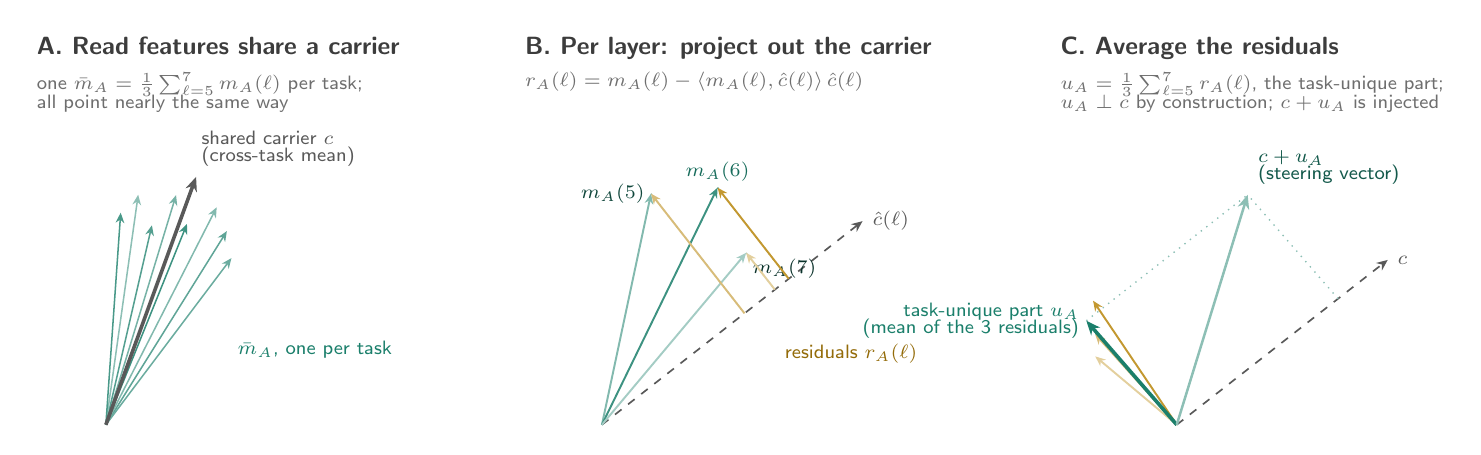
\begin{tikzpicture}[x=1cm,y=1cm]
% ================= Panel A =================
\node[ptitle] at (0,5.45) {A. Read features share a carrier};
\node[small,anchor=north west,align=left] at (0,5.0) {one $\bar m_A=\tfrac13\sum_{\ell=5}^{7} m_A(\ell)$ per task;\\[-1pt]all point nearly the same way};
\coordinate (oA) at (1.0,0.4);
% fan of per-task read features
\foreach \ang/\len/\sh in {58/2.9/70, 63/3.1/55, 68/2.75/85, 73/3.05/60, 77/2.6/75, 82/2.95/50, 86/2.7/80, 53/2.65/65}{
  \draw[thinvec,readc!\sh!white] (oA) -- ++(\ang:\len);
}
% carrier
\draw[vec,line width=1.3pt,gray!70!black] (oA) -- ++(70:3.35) node[pos=1,anchor=south west,small,text=gray!70!black,align=left,xshift=-2pt] {shared carrier $c$\\[-2pt](cross-task mean)};
\node[small,text=readc,anchor=west,align=left] at (2.55,1.35) {$\bar m_A$, one per task};

% ================= Panel B =================
\node[ptitle] at (6.2,5.45) {B. Per layer: project out the carrier};
\node[small,anchor=north west,align=left] at (6.2,5.0) {$r_A(\ell)=m_A(\ell)-\langle m_A(\ell),\hat c(\ell)\rangle\,\hat c(\ell)$};
\coordinate (oB) at (7.3,0.4);
% carrier direction (dashed)
\draw[dashed,gray!70!black,line width=0.6pt,-{Stealth[length=1.4mm,width=1.2mm]}] (oB) -- ++(38:4.2) node[pos=1,anchor=west,small,text=gray!70!black] {$\hat c(\ell)$};
% three per-layer means with their projections
\foreach \ang/\len/\sh/\lbl/\anc in {78/3.0/55/$m_A(5)$/east, 64/3.35/85/$m_A(6)$/south, 50/2.85/40/$m_A(7)$/north west}{
  \coordinate (tip) at ($(oB)+(\ang:\len)$);
  % foot of the projection on the carrier line
  \coordinate (foot) at ($(oB)!(tip)!($(oB)+(38:5)$)$);
  \draw[readc!\sh!white,line width=0.5pt,dotted] (tip) -- (foot);
  \draw[thinvec,readc!\sh!white,line width=0.7pt] (oB) -- (tip) node[pos=1,anchor=\anc,small,text=readc!\sh!black,inner sep=2pt] {\lbl};
}
% residuals r_A(l): perpendicular from foot to tip, drawn from origin translated
\foreach \ang/\len/\sh in {78/3.0/55, 64/3.35/85, 50/2.85/40}{
  \coordinate (tip) at ($(oB)+(\ang:\len)$);
  \coordinate (foot) at ($(oB)!(tip)!($(oB)+(38:5)$)$);
  \draw[thinvec,accentc!\sh!white,line width=0.7pt] (foot) -- (tip);
}
\node[small,text=accentc!80!black,anchor=west,align=left] at (9.5,1.3) {residuals $r_A(\ell)$};

% ================= Panel C =================
\node[ptitle] at (13.0,5.45) {C. Average the residuals};
\node[small,anchor=north west,align=left] at (13.0,5.0) {$u_A=\tfrac13\sum_{\ell=5}^{7} r_A(\ell)$, the task-unique part;\\[-1pt]$u_A\perp c$ by construction; $c+u_A$ is injected};
\coordinate (oC) at (14.6,0.4);
\draw[dashed,gray!70!black,line width=0.6pt,-{Stealth[length=1.4mm,width=1.2mm]}] (oC) -- ++(38:3.4) node[pos=1,anchor=west,small,text=gray!70!black] {$c$};
\foreach \ang/\len/\sh in {132/1.55/55, 124/1.9/85, 140/1.35/40}{
  \draw[thinvec,accentc!\sh!white,line width=0.7pt] (oC) -- ++(\ang:\len);
}
\draw[vec,line width=1.3pt,readc] (oC) -- ++(131:1.75) node[pos=1,anchor=east,small,text=readc,align=right,inner sep=2pt] {task-unique part $u_A$\\[-2pt](mean of the 3 residuals)};
\draw[vec,readc!50!white,line width=0.9pt] (oC) -- ++($(38:2.6)+(131:1.75)$) node[pos=1,anchor=south west,small,text=readc!70!black,align=left] {$c+u_A$\\[-2pt](steering vector)};
\draw[readc!50!white,line width=0.5pt,dotted] ($(oC)+(38:2.6)$) -- ($(oC)+(38:2.6)+(131:1.75)$);
\draw[readc!50!white,line width=0.5pt,dotted] ($(oC)+(131:1.75)$) -- ($(oC)+(38:2.6)+(131:1.75)$);
\end{tikzpicture}
\end{document}
